\documentclass{standalone}

\usepackage{tikz}
\usetikzlibrary{patterns}
\usetikzlibrary{arrows.meta}

\begin{document}

	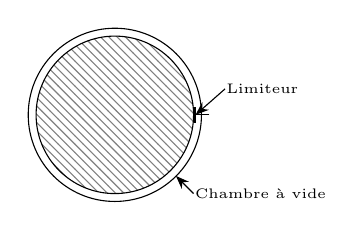
\begin{tikzpicture}

		\fill[pattern=north west lines, pattern color=gray]
    		(0,0) circle [radius=1cm];
		\draw (0,0) circle [radius=1cm];
		
		\draw (0,0) circle [radius=1.1cm];
		
		\draw (1.2, 0) -- (1, 0);
		\fill (1, 0.1) -- (1.025, 0.1) -- (1.025, -0.1) -- (1, -0.1);
		
		\draw[{Stealth}-] (1.1*1.41/2,-1.1*1.41/2) -- (1, -1) node[right=-3pt, align=center] {\tiny\shortstack{Chambre à vide}};
		
		\draw[{Stealth}-] (1.025,0) -- (1.4, 0.33) node[right=-3pt, align=center] {\tiny\shortstack{Limiteur}};
		
	\end{tikzpicture}



\end{document}